%!TEX root = ../root.tex
\section{Data acquisition}

\subsection{Sensors}

Data acquisition was performed with the following four LiDARs: the SICK LMS200, SICK LMS151, Hokuyo UTM-30LX-EW, and the Velodyne HDL-32E. Relevant sensor information is provided in table~\ref{tab:lidars}, but the reader is referred to the manufacturers' documentation for additional information\footnote{Available here: Velodyne~\cite{VelodyneManual}, Hokuyo~\cite{UTMDatasheet}, LMS151~\cite{LMS151Datasheet}, LMS200~\cite{LMS200Manual}}.

The first element that gives a qualitative overview of the sensor performance is the maximum acquisition distance. This value depends on several factors such as lighting conditions and target remission. This value is provided directly for the HDL-32E and UTM-30LX-EW, but based on a target remission greater than \SI{75}{\percent} for the LMS200 and LMS151. Another element to consider is the shape and area covered by the beam, which influences the probability of hitting a snowflake as well as the proportion of area it covers. A final significant element which changes from one sensor to the other is the number of echoes returned. The Hokuyo sensor can return up to three echoes, which means that it could locate two snowflakes before the beam reaches the ground. Regarding the LMS151, two echoes are evaluated by the hardware, but only one is returned. Finally, note that all LiDARs use class 1 laser with a wavelength of \SI{905}{\nano\meter}. This wavelength part of the solar spectrum, which means that outdoor lighting conditions could potentially cause interference.

\begin{table*}[htbp]
    \centering
    % \def\tabularxcolumn#1{m{#1}}
    \begin{tabular}{|c|c|c|c|c|}
        \hline
        \textbf{Sensor}     & \textbf{Maximum distance}  & \textbf{Spot area (at 30 meters)}  & \textbf{Spot shape} & \textbf{Echoes} \\\hline
        SICK LMS200         & \SI{28}{\meter}            & \SI{165}{\centi\meter\squared}     & Circle              & 1               \\\hline
        SICK LMS151         & \SI{50}{\meter}            & \SI{22}{\centi\meter\squared}      & Circle              & 2               \\\hline
        Hokuyo UTM-30LX-EW  & \SI{30}{\meter}            & \SI{196}{\centi\meter\squared}     & Ellipse             & 3               \\\hline
        Velodyne HDL-32E    & \SI{70}{\meter}            & \SI{51}{\centi\meter\squared}      & Rectangle           & 1               \\\hline
    \end{tabular}
    \caption{Overview of characteristics specific to each LiDAR.}
    \label{tab:lidars}
\end{table*}

\subsection{Setup configuration}

Data acquisition was conducted at Pouliot Hall of Laval University, where sensors were placed close to the inner wall of a window facing N\SI{50}{\degree}E. As shown in fig.~\ref{fig:setup}, a wooden structure held the sensors side by side at approximately \SI{13.9}{\meter} above the ground and the main scanning plane (i.e. XY plane in the sensor reference frame) formed a \SI{30}{\degree} angle with respect to the building wall. In addition, an RGB camera was placed alongside the LiDARs to provide visual information about the scene. In this configuration, a slight opening of the window allowed to keep the instruments inside while scanning outside. To avoid direct interference between sensors, corrugated plastic layers were placed between them.

Fig.~\ref{fig:view} shows the scene as observed by the RGB camera placed with the sensors. In particular, the second row of fig.~\ref{fig:view} shows how the building casts a shadow that progressively covers the scene over the course of the day. This will allow us to explore the influence of lighting, as well as snow in sec.~\ref{sec:data-analysis}.

\begin{figure}[th]
    \centering
    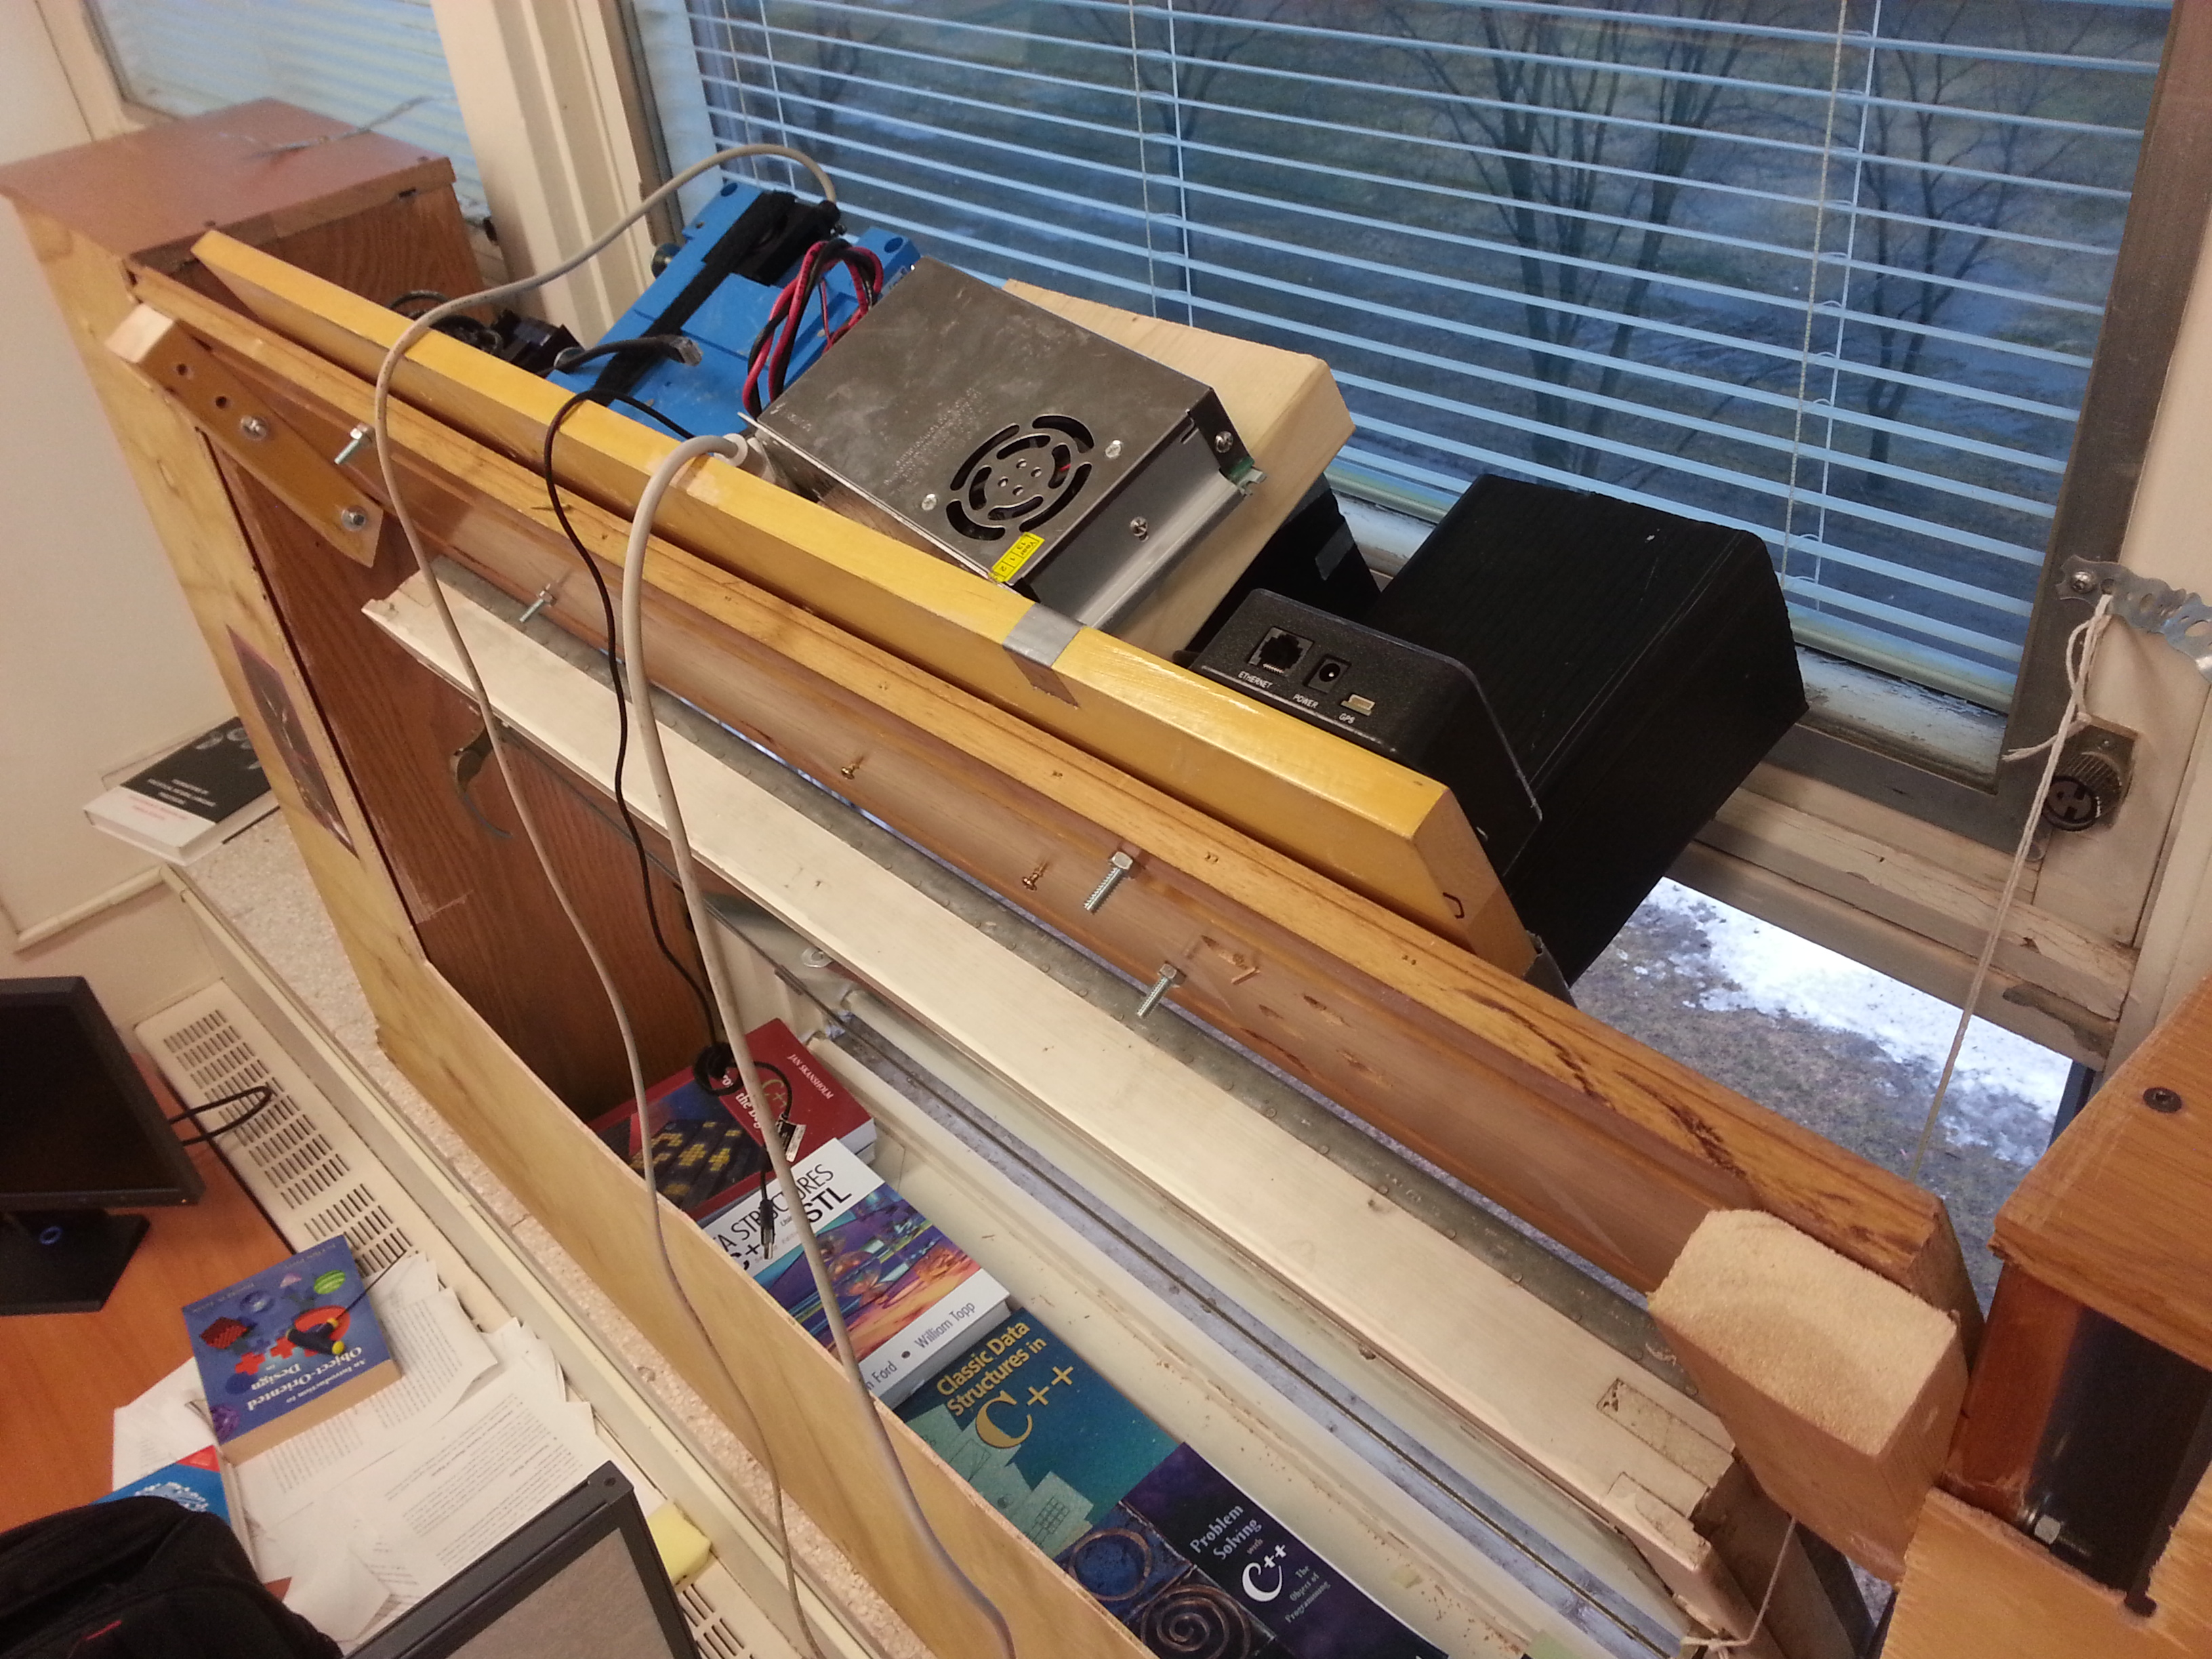
\includegraphics[width=0.95\linewidth]{./img/setup_diag.png}
    \caption{The experimental setup. The 3D axis represent the orientation of the sensors and the bottom left panel represent the 2D geometry as seen from the right side of the picture.}
    \label{fig:setup}
\end{figure}

\begin{figure}[th]
    \centering
    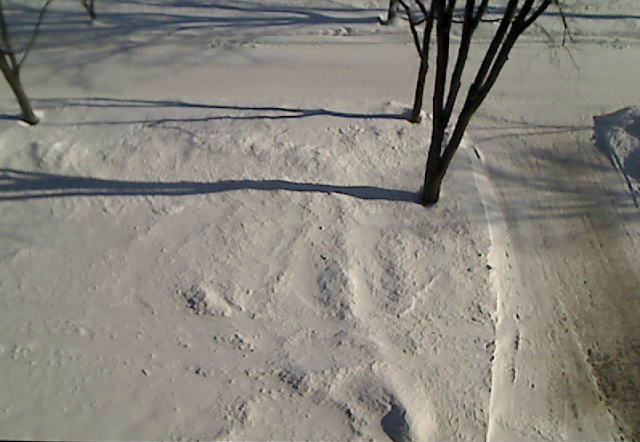
\includegraphics[width=0.90\linewidth]{./img/camera_view.jpg}\\*[.5em]
    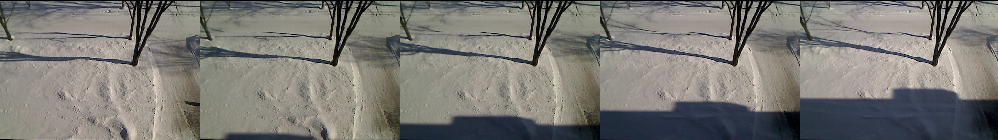
\includegraphics[width=0.90\linewidth]{./img/shadow2.png}
    \caption{View from the RGB camera. The sequence of pictures at the bottom shows the evolution of the shadow caused by the building between 10:00~am and 10:40~am.}
    \label{fig:view}
\end{figure}

\subsection{Dataset description} % TODO change number of acquisitions and overall time if required (and check abstract also)
Data acquisition started February~11 and ended on March~21. A total of 14 samples were obtained for a total of more than 78 hours of data. Recordings were made using the Robot Operating System (ROS)~\cite{ROSWeb}, which provides standardized data types as well as time synchronization. Data was acquired at different times of day and in a wide variety of conditions, covering a wide range of snowflakes size, falling rate, sky type and wind speed. The target ground area also changed from different amount and type of snow to complete grass. Table~\ref{tab:overview-dataset} provides an overview of our data\footnote{Wind speed, daily precipitation and temperature are reported from Québec City Jean Lesage International Airport at approximately \SI{9}{\km} from Laval University. Data is available here \cite{WeatherCanada}.}. The dataset will be publicly available upon paper acceptance.

\begin{table*}[htbp]
    \centering
    \todo{Confirm that this table is ok (delete unwanted information and correct errors)}\\
    \todo{Why do we have ``night'' as a sky type?}\\
    \todo{Should we exclude the first day as it only has 6 minutes?}
    \todo{Shoudl we exclude the days with no snow?}
    \begin{tabular}{|c|c|c|c|c|c|c|c|}
        \hline
        \textbf{Beginning} & \textbf{Duration} & \textbf{Sky}  & \textbf{Snowflakes} & \textbf{Falling} & \textbf{Wind speed range}      & \textbf{Daily precipitation}  & \textbf{Temperature}     \\
        \textbf{time}      & \textbf{(HH:MM)}  & \textbf{type} & \textbf{size}       & \textbf{rate}    & \textbf{(\SI{}{\km\per\hour})} & snow/\textit{rain}            & \textbf{(\SI{}{\celsius})}      \\\hline
        Feb 11, 8:46 am    &  00:06            & Night         & Small               & Low/medium       & [16-18]                        & \SI{1}{\cm}                   & -17.4 \\\hline
        Feb 12, 9:47 am    &  09:21            & Cloudy        & Small               & Variable         & [2-13]                         & \SI{1.4}{\cm}                 & -14.1 \\\hline
        Feb 14, 10:12 pm   &  04:12            & Night         & Small               & Very low         & [5-13]                         & \SI{0.2}{\cm}                 & -21.4 \\\hline
        Feb 16, 12:27 pm   &  07:17            & Clear         & None                & None             & [14-29]                        & \SI{0}{\cm}                   & -15.5 \\\hline
        Feb 17, 12:02 pm   &  24:36            & Cloudy        & None                & None             & [1-9]                          & \SI{0}{\cm}                   & -20.2 \\\hline
        Feb 19, 8:38 am    &  10:02            & Cloudy        & Big/small           & High             & [3-28]                         & \SI{4.5}{\cm}                 & -10.9 \\\hline
        Mar 2, 1:06 pm     &  01:27            & Cloudy        & Big/small           & Variable         & [22-36]                        & \SI{1.6}{\cm}                 & -9.1  \\\hline
        Mar 3, 10:33 pm    &  02:17            & Night         & Big                 & Medium           & [7-9]                          & \SI{5.4}{\cm}                 & -13.3 \\\hline
        Mar 4, 11:45 am    &  04:12            & Cloudy        & Big/medium          & Low/none         & [20-30]                        & \SI{2.0}{\cm}                 & -4.3  \\\hline
        Mar 17, 10:08 am   &  06:08            & Cloudy        & Big/medium          & Low/none         & [1-31]                         & \SI{2.0}{\cm}                 & -5.8  \\\hline
        Mar 21, 6:44 pm    &  07:42            & Night         & Medium/big          & High             & [5-33]                         & \SI{8.6}{\cm}                 & -5.1  \\\hline
        Mar 30, 1:06 pm    &  04:45            & Cloudy        & Medium/big          & High             & [4-8]                          & \SI{8.5}{\cm}                 & -3.0  \\\hline
        Apr 2, 1:56 pm     &  01:51            & Cloudy        & Small/rain          & High             & [2-10]                         & \SI{1.2}{\cm}/\textit{5.4 mm} & -8.4  \\\hline
        Apr 21, 10:52 am   &  01:39            & Cloudy        & Rain                & Medium           & [16-18]                        & \textit{15 mm}                & 14.6  \\\hline
    \end{tabular}
    \caption{Overview of our snow dataset.}
    \label{tab:overview-dataset}
\end{table*}

